\subsection{Немного практики}

\begin{frame}{Упражнения}
	\begin{enumerate}
		\item Скачайте файл \href{https://www.dropbox.com/s/jo26qgwysxsb8aj/literacy.sql?dl=0}{literacy.sql}.
		\item Выберите имя для файла, где у вас будет лежать БД для тестов (например, \t{literacy.sqlite3}.
		\item Выполните запросы из \t{literacy.sql}:
			\begin{center}
				\t{sqlite3 literacy.sqlite3 < literacy.sql}
			\end{center}
			Каждый раз, когда вы будете выполнять команды из \t{literacy.sql}, таблицы
			будут полностью пересозданы.
			Не бойтесь что-то сломать.
		\item
		     Выполните SQL-запросы (либо в командной строке, либо в GUI):
		     \begin{enumerate}
		     	\item Всю информацию по всем странам.
		     	\item Первые десять стран (если сортировать по названию).
		     	\item Средние население и площадь страны.
		     	\item Площадь и население Франции.
		     	\item Количество французских территорий и их суммарную площадь и население.
		     \end{enumerate}
	\end{enumerate}
\end{frame}

\begin{frame}{NULL}
	Также есть специальное значение \t{NULL}, которое может лежать в любой колонке, если только на ней нет ограничения \t{NOT NULL}.
	Может обозначать:
	\begin{itemize}
		\item Отсутствие каких-либо данных (неизвестно население страны).
		\item Неопределённый результат вычисления (среднее значение пустого множества, деление на ноль).
		\item Что угодно ещё по желанию программиста.
	\end{itemize}
	Возникающая проблема: нет одного объяснения, как \t{NULL} себя ведёт в разных запросах.
	\begin{itemize}
		\item
			Если считать, что \t{NULL} распространяется как \t{NaN} (Not a Number), т.е. любое вычисление с \t{NULL} даёт \t{NULL},
			то сложно писать запросы в ситуации, где наличие \t{NULL} "--- норма.
		\item
			Если \t{NULL} просто игнорировать, то про него легко забыть (так часто и делают); а он может где-то требовать специальной обработки.
	\end{itemize}
\end{frame}

\begin{frame}{Демонстрация NULL}
    \begin{itemize}
    	\item Разные функции обрабатывает \t{NULL} по-разному, общая цель "--- наиболее консистентное и адекватное поведение.
    	\item Обычно в агрегирующих функциях игнорируется.
    	\item Если вы пишете чуть-чуть несимметричный код (вроде \t{SUM(a) / COUNT(*)}), могут быть последствия.
    	\item Очень легко забыть и получить какой-то правдоподобный, но неверный результат (особенно в соединениях "--- будут дальше).
    \end{itemize}
\end{frame}

\begin{frame}[t,fragile]{SQL-инъекции}
	Пусть есть таблица с полями: владелец текста, его название, содержимое.
	Код для доступа к базе, выполняется на сервере:
\begin{minted}{python}
with sqlite3.Connection("sql-injection.sqlite3") as db:
  key = input('Text key: ')
  cursor = db.execute("""SELECT * FROM Text
                         WHERE owner='user' AND key='{}'"""
                         .format(key))
  print(list(cursor))
\end{minted}
	\only<1-2>{
	В чём проблема?
	\only<2>{
	\begin{center}
		\begin{tabular}{ll}
			Значение: & \t{key1} \\\hline
			Было:  & \t{SELECT ... WHERE owner='user' AND key='\{\}'} \\\hline
			Стало: & \t{SELECT ... WHERE owner='user' AND key='key1'} \\
		\end{tabular}
	\end{center}
	}
	}
	\only<3-4>{
	К коллайдеру!
	\only<4>{
	\begin{center}
		\begin{tabular}{ll}
			Значение: & \t{' OR ''='} \\\hline
			Было:  & \t{SELECT ... WHERE owner='user' AND key='\{\}'} \\\hline
			Стало: & \t{SELECT ... WHERE owner='user' AND key='' OR ''=''} \\
		\end{tabular}
	\end{center}
	}
	Упс.
	}
\end{frame}

\begin{frame}{Классический комикс}
	\begin{center}
		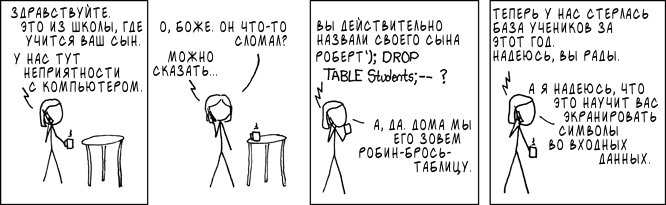
\includegraphics[scale=0.5]{xkcd-327.png}
	\end{center}
\end{frame}

\begin{frame}[fragile]{А как правильно?}
\begin{minted}{python}
with sqlite3.Connection("sql-injection.sqlite3") as db:
  key = input('Text key: ')
  cursor = db.execute("SELECT * FROM Text WHERE owner='user' AND key=?", [key])
  print(list(cursor))
\end{minted}
	Теперь драйвер базы данных знает, что \t{key} "--- это значение от пользователя,
	которое надо \textit{заэкранировать}:
	\begin{center}
		\begin{tabular}{ll}
			Значение: & \t{' OR ''='} \\\hline
			Было:  & \t{... WHERE owner='user' AND key=?} \\\hline
			Стало: & \t{... WHERE owner='user' AND key='\textbackslash' OR  \textbackslash'\textbackslash'=\textbackslash''} \\
		\end{tabular}
	\end{center}
	Независимо от того, какой код мы напишем, SQL-инъекции не случится.

	Мораль: никогда не собирайте SQL-запрос руками из переменных.
\end{frame}
